% This LaTeX document needs to be compiled with XeLaTeX.
\documentclass[10pt]{article}
\usepackage{graphicx}
\usepackage[export]{adjustbox}
\graphicspath{ {./images/} }
\usepackage[fallback]{xeCJK}
\usepackage{polyglossia}
\usepackage{fontspec}
\setCJKmainfont{Noto Serif CJK JP}

\setmainlanguage{polish}
\setmainfont{CMU Serif}

\title{LIGA MATEMATYCZNA \\
 FINAモ \\
 26 marca 2010 \\
 SZKOŁA PODSTAWOWA }

\author{}
\date{}


\begin{document}
\maketitle
\section*{ZADANIE 1.}
Dziesięć pająków zjada dziesięć much w ciągu dwudziestu sekund. Ile czasu potrzeba stu pająkom na zjedzenie stu much?

\section*{ZADANIE 2.}
Suma trzynastu różnych liczb całkowitych dodatnich jest równa 92. Wyznacz te liczby.

\section*{ZADANIE 3.}
Kamila, Ania i Marek twierdzą, że suma ich lat jest równa 35. Jednak żadne z nich nie podało prawdziwego wieku. Kamila zaniżyła swój wiek o 3 lata, Ania zawyżyła o 2 lata, a Marek postarzył się o 4 lata. Kiedy naprawdę suma ich lat będzie równa 35 ?

\section*{ZADANIE 4.}
Ślimak wspina się na drzewo o wysokości 10 m . W ciągu dnia podnosi się o 4 metry, a w nocy obsuwa się o 3 metry. Po ilu dniach ślimak dostanie się na wierzchołek drzewa?

\section*{ZADANIE 5.}
Prostokąt podzielono na dziewięć różnych kwadratów (rysunek na odwrocie). Długość boku najmniejszego kwadratu jest równa 1.\\
(a) Znajdź długość boku zamalowanego kwadratu.\\
(b) Znajdź długości boków prostokąta.\\
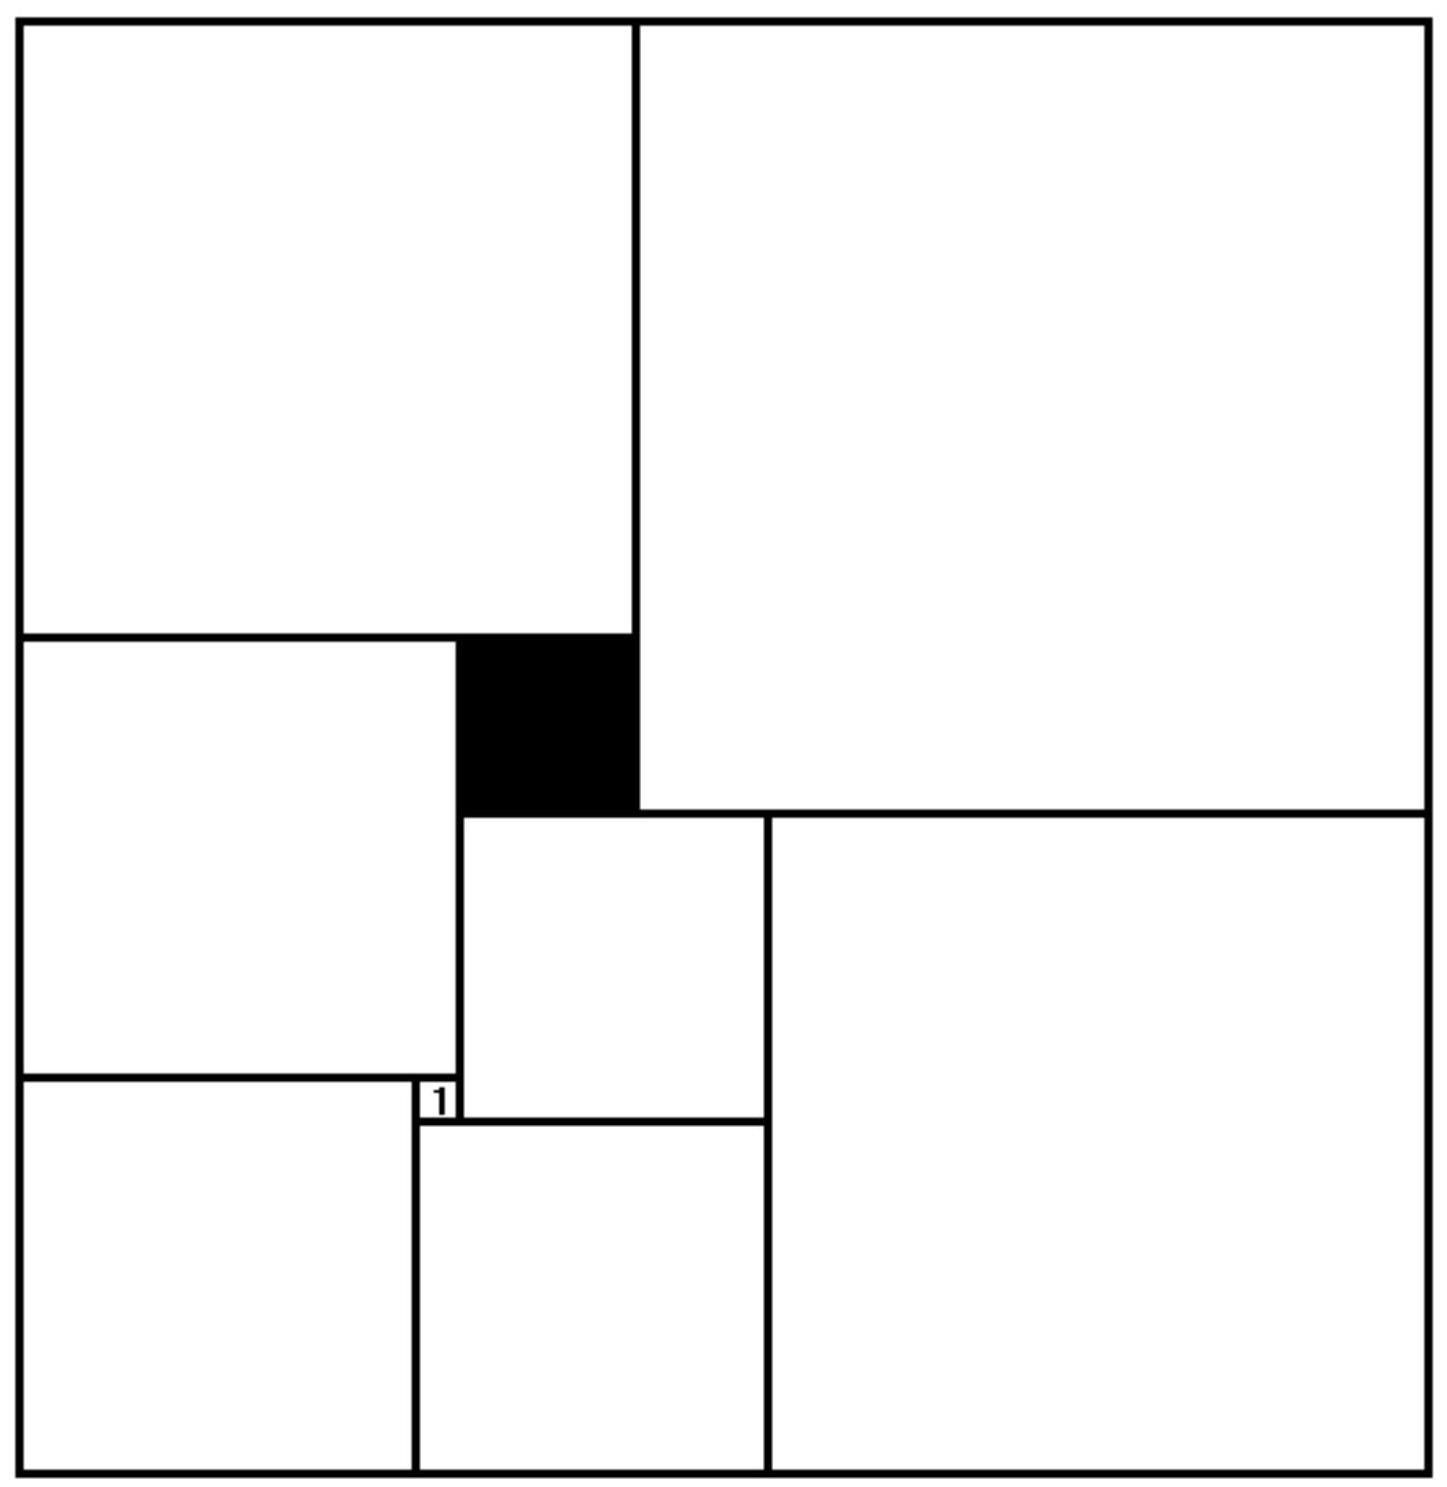
\includegraphics[max width=\textwidth, center]{2024_11_21_26b6528d4939a170073ag-2}


\end{document}